
\documentclass[10pt]{article}

% PLoS Required Packages
\usepackage{graphicx}
\usepackage{cite}
\usepackage{color}

% Text layout
\topmargin 0.0cm
\oddsidemargin 0.5cm
\evensidemargin 0.5cm
\textwidth 16cm 
\textheight 21cm

% Bold the 'Figure #' in the caption and separate it with a period
% Captions will be left justified
\usepackage[labelfont=bf,labelsep=period,justification=raggedright]{caption}

% Other packages
\usepackage{fancyhdr}
\usepackage[utf8]{inputenc}
\usepackage{float}

% Commands to make things easier and set lengths
\newcommand{\de}{$^\circ$} % \ensuremath kills latex2png
\addtolength{\parskip}{\baselineskip}
\setlength{\parindent}{0in}

% Set short title as running header
\pagestyle{fancy}
\lhead{Cross-bridge forces depend on lattice spacing}
\rhead{PLoS Comp Biol}
\cfoot{ }
\renewcommand{\headrulewidth}{0pt}

\date{} % Leave date blank

% header (end)

\begin{document}

\begin{figure}[!ht]
    \begin{center}
    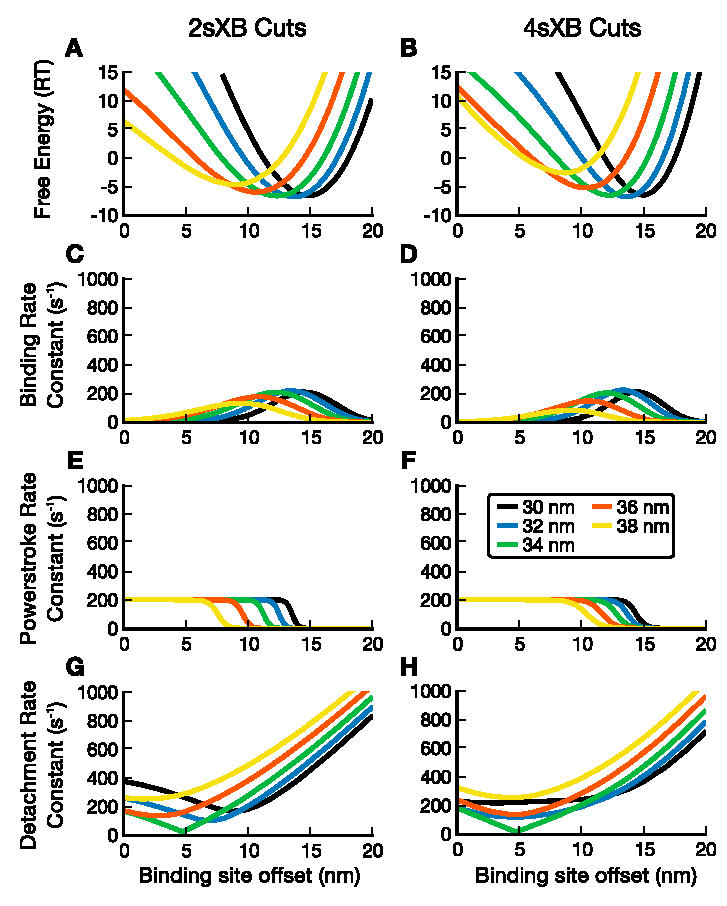
\includegraphics[height=.8\textheight]{./fig_multiple_kinetics_cuts.pdf}
    \parbox{\textwidth}{
        \vspace{1em}
        \textbf{Figure S2: Cross-bridge free energy and kinetics at multiple lattice spacings}
        (A)--(B) show the free energies of the 4sXB and the 2sXB models at lattice spacings between 30 and 38 nm. 
        (C)--(H) show the kinetic rate constants of the 4sXB and the 2sXB models at lattice spacings between 30 and 38 nm.
        Each rate is a section taken from the corresponding display in Figure 3. %\ref{fig_kinetics_contours}.
        \label{fig_multiple_kinetics_cuts}
        }
    \end{center}
\end{figure}

\end{document}
